% BGIN Block 15 — the IKP co-chair's four sessions (15–16 Oct 2026, Georgetown University Capitol Campus)
% 1-4 / 1-7 PQC Migration (Room B, 15 Oct 09:50–13:00) · 2-6 Privacy Enhanced Authentication, ZKP & Proof of
% Personhood (Room B, 16 Oct 11:30–13:00) · 2-9 AML Policy, Forensics & Analytics — Common Taxonomy (FASE/IKP,
% Room A, 16 Oct 15:40–17:10, with Chloe White).
% House style of the GDC26 / Block 15 PQC decks: dark title bar, grey lead box, "Takeaway" line, BGIN mark in the footer.
% Facts follow the Block 15 programme (bgin-global.org/events/20261015-block15), bgin-global/pqc-agility-competition
% (draft v0, main 86c780a), the Block 14 meeting reports, the proof-of-human convergence note (Aug 2026) and the
% IKP KB in ~/BGIN_IKP. Everything shown is unratified.
% Build: latexmk -pdf Block15_IKP_CoChair_Sessions.tex
\documentclass[aspectratio=169,10pt]{beamer}
\usepackage[utf8]{inputenc}
\usepackage[T1]{fontenc}
\usepackage{helvet}
\renewcommand{\familydefault}{\sfdefault}
\usepackage{booktabs}
\usepackage{array}
\usepackage{graphicx}
\usepackage{fontawesome5}
\usepackage{tikz}
\usetikzlibrary{arrows.meta,positioning,calc}
\usepackage{qrcode}
\usepackage{hyperref}

\usetheme{default}
\setbeamersize{text margin left=7mm,text margin right=7mm}
\setlength{\tabcolsep}{4pt}
\definecolor{bar}{RGB}{25,25,29}
\definecolor{ink}{RGB}{35,35,40}
\definecolor{soft}{RGB}{110,110,118}
\definecolor{boxbg}{RGB}{242,242,244}
\definecolor{lane}{RGB}{225,227,232}
\definecolor{pqc}{RGB}{247,147,26}
\definecolor{pop}{RGB}{92,74,140}
\definecolor{popbg}{RGB}{236,233,244}
\definecolor{aml}{RGB}{18,108,108}
\definecolor{amlbg}{RGB}{228,240,239}
\setbeamercolor{normal text}{fg=ink}
\setbeamercolor{structure}{fg=bar}
\setbeamercolor{frametitle}{bg=bar,fg=white}
\setbeamercolor{block body}{bg=boxbg,fg=ink}
\setbeamercolor{pop body}{bg=popbg,fg=ink}
\setbeamercolor{aml body}{bg=amlbg,fg=ink}
\setbeamertemplate{navigation symbols}{}
\setbeamertemplate{itemize item}{\color{bar}\faAngleRight}
\setbeamertemplate{itemize subitem}{\color{soft}\textendash}
\setbeamertemplate{enumerate item}{\colorbox{bar}{\color{white}\scriptsize\insertenumlabel}}
\setbeamerfont{frametitle}{series=\bfseries,size=\large}
\setbeamertemplate{frametitle}{%
  \vskip-2pt\begin{beamercolorbox}[wd=\paperwidth,ht=8mm,dp=2.5mm,leftskip=6mm]{frametitle}%
  \usebeamerfont{frametitle}\insertframetitle\hfill{\small\mdseries\insertframesubtitle}\hspace{6mm}\end{beamercolorbox}}
\setbeamertemplate{footline}{%
  \begin{beamercolorbox}[wd=\paperwidth,ht=5mm,dp=2mm,leftskip=6mm,rightskip=6mm]{normal text}%
  \tiny\color{soft}\raisebox{-1.2pt}{
\includegraphics[height=3.2mm]{bgin_mark.png}}\hspace{1.2mm}%
  BGIN Block 15 --- FASE/IKP 2-9: AML Policy, Forensics \& Analytics\hfill Washington, D.C. \textbar{} 16 Oct 2026, 15:40 / \insertframenumber\end{beamercolorbox}}
\newcommand{\takeaway}[1]{\par\vspace{1.5mm}{\small\color{bar}\faLink~\textbf{Takeaway:} #1}}
\newcommand{\lead}[1]{\begin{beamercolorbox}[wd=\textwidth,sep=2.5mm]{block body}\small #1\end{beamercolorbox}\par\vspace{2mm}}
\newcommand{\poplead}[1]{\begin{beamercolorbox}[wd=\textwidth,sep=2.5mm]{pop body}\small #1\end{beamercolorbox}\par\vspace{2mm}}
\newcommand{\amllead}[1]{\begin{beamercolorbox}[wd=\textwidth,sep=2.5mm]{aml body}\small #1\end{beamercolorbox}\par\vspace{2mm}}
\newcommand{\pillar}[3]{\begin{minipage}[t]{#1}\colorbox{bar}{\parbox{\dimexpr\linewidth-2\fboxsep}{\color{white}\small\textbf{#2}}}\par\vspace{1mm}{\small #3}\end{minipage}}
\newcommand{\cpillar}[4]{\begin{minipage}[t]{#2}\colorbox{#1}{\parbox{\dimexpr\linewidth-2\fboxsep}{\color{white}\small\textbf{#3}}}\par\vspace{1mm}{\small #4}\end{minipage}}
% \sectiontitle{accent}{kicker}{title}{subtitle}
\newcommand{\sectiontitle}[4]{{\setbeamertemplate{footline}{}\begin{frame}[plain]
  \begin{tikzpicture}[remember picture,overlay]
    \fill[bar] (current page.north west) rectangle (current page.south east);
    \node[anchor=north east,inner sep=0] at ([xshift=-7mm,yshift=-5mm]current page.north east){
\includegraphics[height=1.9cm]{bgin_logo.png}};
    \node[anchor=south west,text=#1,font=\small\bfseries] at ([xshift=7mm,yshift=-2.9cm]current page.north west){#2};
    \node[anchor=south west,text=white,font=\Large\bfseries,text width=13cm,align=left] at ([xshift=7mm,yshift=-4.7cm]current page.north west){#3};
    \node[anchor=north west,text=white,font=\small,text width=13cm,align=left] at ([xshift=7mm,yshift=-5.0cm]current page.north west){#4};
  \end{tikzpicture}
\end{frame}}}
\hypersetup{colorlinks,urlcolor=bar,linkcolor=ink}
\newcommand{\nohyph}{\hyphenpenalty=10000 \exhyphenpenalty=10000 \relax}

\begin{document}

% ================================================================ TITLE
{\setbeamertemplate{footline}{}
\begin{frame}[plain,t]
  \begin{tikzpicture}[remember picture,overlay]
    \fill[bar] (current page.north west) rectangle ([yshift=-3.5cm]current page.north east);
    \node[anchor=north east,inner sep=0] at ([xshift=-7mm,yshift=-5mm]current page.north east){
\includegraphics[height=1.9cm]{bgin_logo.png}};
    \node[anchor=west,text=white,font=\Large\bfseries,text width=11.2cm,align=left] at ([xshift=7mm,yshift=-1.35cm]current page.north west){AML Policy, Forensics \& Analytics --- a Common Taxonomy};
    \node[anchor=west,text=aml,font=\small,text width=11.2cm,align=left] at ([xshift=7mm,yshift=-2.85cm]current page.north west){Joint FASE / IKP session 2-9 \textperiodcentered{} the \emph{Forensics \& Analysis} document in public comment, and the common lexicon of harmful on-chain activities};
    \node[anchor=west,font=\normalsize,text width=13.2cm] at ([xshift=7mm,yshift=-4.6cm]current page.north west){Mitchell Travers (Co-Chair, IKP) \textperiodcentered{} Chloe White (Co-Chair, FASE)};
    \node[anchor=north west,font=\small,text=soft,text width=13.2cm,align=left] at ([xshift=7mm,yshift=-5.0cm]current page.north west){BGIN Block \#15 \textbar{} Georgetown University Capitol Campus, Washington, D.C. \textbar{} 16 October 2026, Room A, 15:40--17:10 \textbar{} hybrid};
    \node[anchor=west,font=\scriptsize,text=soft,text width=13cm,align=left] at ([xshift=7mm,yshift=-6.5cm]current page.north west){Continues the Block 14 joint session \emph{Forensics \& Analysis --- Common Lexicon of Harmful Activities} (Tokyo, March 2026) \textperiodcentered{} the lexicon records typologies and signals, not verdicts; no tool, vendor or jurisdiction is endorsed};
  \end{tikzpicture}
\end{frame}}

% ================================================================ CONTEXT
\begin{frame}{This Session --- What It Is For}
  \amllead{Review the comments received on the public-comment document, settle the forensics-versus-analytics framing, advance the common lexicon, agree what guidance VASPs, investigators and educators need, and ask what can be inferred, by whom, with what safeguards.}
  \begin{enumerate}\footnotesize\setlength{\itemsep}{0.5mm}
    \item The Forensics \& Analysis document in public comment: review of comments received
    \item Forensics versus analytics: settling the common framing
    \item The illicit-activity common lexicon: terms in progress and how practitioners and policymakers use them
    \item Guidance for VASPs, investigators and educators
    \item Privacy and proportionality in analytics: what can be inferred, by whom, and with what safeguards
    \item Next steps toward publication
  \end{enumerate}
  \takeaway{Leave with comment dispositions, the framing settled as the document's first section, and the lexicon's v1 scope and record shape.}
\end{frame}

% ================================================================ 28 where it came from
\begin{frame}{Where This Work Came From}
  \begin{center}
  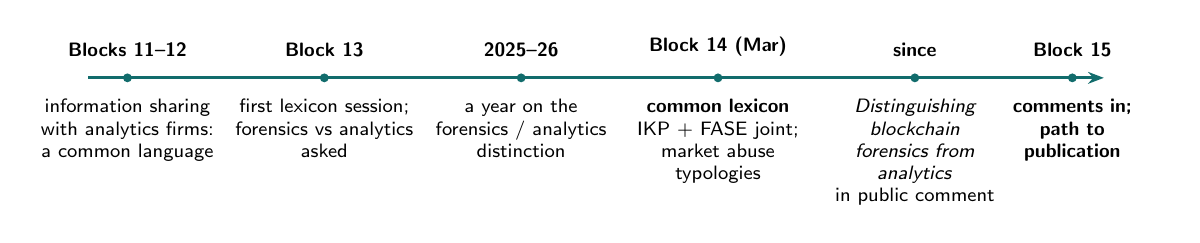
\begin{tikzpicture}[font=\scriptsize]
    \draw[line width=1pt,aml,-{Stealth[length=2mm]}] (0,0) -- (12.9,0);
    \foreach \x/\lab/\txt in {
      0.5/Blocks 11--12/{information sharing\\ with analytics firms:\\ a common language},
      3.0/Block 13/{first lexicon session;\\ forensics vs analytics\\ asked},
      5.5/2025--26/{a year on the\\ forensics / analytics\\ distinction},
      8.0/Block 14 (Mar)/{\textbf{common lexicon}\\ IKP + FASE joint;\\ market abuse typologies},
      10.5/since/{\emph{Distinguishing blockchain}\\ \emph{forensics from analytics}\\ in public comment},
      12.5/Block 15/{\textbf{comments in;}\\ \textbf{path to}\\ \textbf{publication}}}
      {\fill[aml] (\x,0) circle (1.6pt);
       \node[above=1.5mm,align=center,font=\scriptsize\bfseries] at (\x,0) {\lab};
       \node[below=1.5mm,align=center,text width=2.3cm] at (\x,0) {\txt};}
  \end{tikzpicture}
  \end{center}
  \par\vspace{2mm}
  \amllead{Two outcomes were asked for at Block 14: a \textbf{common language} (and possibly a shared database) for what practitioners see, and \textbf{getting the terminology right} between what is analytic understanding of chain data and what can stand as forensic evidence in court. Both are served by one lexicon.}
  \takeaway{The problem was never a lack of definitions. It is the cacophony of them.}
\end{frame}

% ================================================================ 29 forensics vs analytics
\begin{frame}{Forensics versus Analytics --- Settling the Framing}
  \begin{center}\scriptsize
  \begin{tabular}{@{}p{2.9cm}p{5.3cm}p{5.5cm}@{}}\toprule
     & \textbf{Blockchain analytics} & \textbf{Blockchain forensics}\\ \midrule
    Question answered & What is probably happening, at scale, now? & What happened, in this case, provably?\\
    Nature of the output & Probabilistic: heuristics, clustering, risk scores, typology matches & Evidentiary: attribution, chain of custody, reproducible method, documented limits\\
    Standard it meets & Fitness for a compliance or surveillance decision & Admissibility: reliability of method, error rate, expert testimony precedents\\
    Who uses it & VASPs, surveillance vendors, supervisors, researchers & Investigators, prosecutors, courts, counsel, regulators in enforcement\\
    Data it rests on & On-chain plus off-chain (venue, news, social); most activity is still off-chain & The same, with provenance of every input recorded\\
    Failure mode & False positives at scale; proprietary and unexplained signals & Over-claiming certainty from a probabilistic tool\\ \bottomrule
  \end{tabular}
  \end{center}
  {\scriptsize\color{soft} Precedents for probabilistic methods in evidence already exist (DNA matching, facial recognition), including how error rates and disclosure duties were handled.}
  \takeaway{Analytics generates leads; forensics proves. A document that says which one a tool is doing, and when a result crosses from one to the other, is the deliverable.}
\end{frame}

% ================================================================ 30 lexicon in progress
\begin{frame}{The Common Lexicon --- Terms in Progress}
  \amllead{Block 14 started from market abuse, where the typologies are most crypto-specific and the data is richest; AML/CFT terms, where much is not unique to crypto, are mapped rather than redefined.}
  \begin{center}\scriptsize
  \begin{tabular}{@{}p{2.4cm}p{5.0cm}p{6.4cm}@{}}\toprule
    \textbf{Family} & \textbf{Terms in progress} & \textbf{Observed signal}\\ \midrule
    Market abuse & Insider trading; pump and dump, incl. cross-venue pumps; touting (social or news driven) & Pre-announcement accumulation on-chain (one survey: clear signals in 56\% of listings studied); 15-minute venue pumps; off-chain news as data\\
    Scams by construction & Hard-coded rug pull; honeypot; related sub-typologies & Contract code present at deployment that has no legitimate purpose; detectable at the moment of deployment\\
    Wash trading & A-to-A; multi-party; cross-symbol (prediction markets) & Non-economic trading in swap pools and order books; the term was built for central limit order books and has to be re-defined for pools\\
    AML / CFT & Sanctions exposure; laundering through non-economic trading; mixing & More binary than market abuse: touched the sanctioned actor or did not. Maps to FATF, FinCEN red-flag advisories and national rules rather than inventing terms\\ \bottomrule
  \end{tabular}
  \end{center}
  {\scriptsize\color{soft} ``One person's wash trading is another's launch strategy.'' Market-abuse lines are drawn by law and settled by courts; the lexicon records the typology and the signal, not the verdict.}
  \takeaway{Mapping first, defining second: what definitions exist (ISO TC 307 vocabulary, FATF, national rules), where they conflict, and only then where a new term is needed.}
\end{frame}

% ================================================================ 31 machine-readable
\begin{frame}{From Lexicon to Something Machines Can Use}
  \begin{center}
  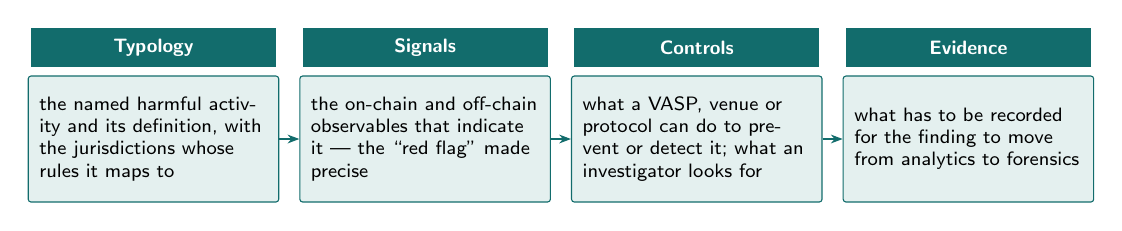
\begin{tikzpicture}[font=\scriptsize, box/.style={draw=aml,fill=amlbg,rounded corners=1pt,text width=2.9cm,align=left,inner sep=4pt,minimum height=1.6cm}, hd/.style={fill=aml,text=white,font=\scriptsize\bfseries,text width=2.9cm,align=center,inner sep=3pt,minimum height=5mm}]
    \foreach \i/\h/\t in {0/Typology/{the named harmful activity and its definition, with the jurisdictions whose rules it maps to},1/Signals/{the on-chain and off-chain observables that indicate it --- the ``red flag'' made precise},2/Controls/{what a VASP, venue or protocol can do to prevent or detect it; what an investigator looks for},3/Evidence/{what has to be recorded for the finding to move from analytics to forensics}}
      {\node[hd] (h\i) at (\i*3.45,0) {\h};
       \node[box,below=1mm of h\i] (b\i) {\t};}
    \foreach \i/\j in {0/1,1/2,2/3} \draw[-{Stealth[length=1.5mm]},aml] (b\i.east) -- (b\j.west);
  \end{tikzpicture}
  \end{center}
  \par\vspace{1.5mm}
  \begin{itemize}\small
    \item The shape of a \textbf{national vulnerability database}, for crypto harms: the Block 14 room pointed at the MITRE framework for crypto-specific exploitation as the nearest published precedent, and at BGIN's own cybersecurity information-sharing framework as the ``securitised'' sibling.
    \item \textbf{Formal over natural language where possible}: an ISO vocabulary standard takes three to four years; a standard that categorises a method or a mathematical object moves faster (the ISO 29128 experience).
    \item \textbf{Proprietary signals}: analytics firms may not disclose detection logic; the lexicon records typology and signal class, not vendor heuristics.
  \end{itemize}
  \takeaway{Two liaison organisations pushing the same taxonomy into ISO TC 307 is more impactful than one. BGIN is Category A; the mapping exercise is the lever.}
\end{frame}

% ================================================================ 32 privacy & proportionality
\begin{frame}{Privacy and Proportionality --- Inference and Its Limits}
  \amllead{A public ledger makes inference cheap. The question is not whether analytics is possible but what inferences are proportionate to the purpose, who may draw them, and what the subject can contest.}
  \begin{columns}[T]
    \begin{column}{0.48\textwidth}
      {\small\textbf{Three questions for every analytic}}
      \begin{itemize}\small
        \item \textbf{What} is inferred --- an address cluster, a counterparty, a person, a pattern of life?
        \item \textbf{By whom}, under what authority --- a VASP meeting its obligations, a vendor, a supervisor, law enforcement with process?
        \item \textbf{With what safeguards} --- retention, purpose limitation, error-rate disclosure, a route to contest a false positive?
      \end{itemize}
    \end{column}
    \begin{column}{0.48\textwidth}
      {\small\textbf{Where it meets this morning's session}}
      \begin{itemize}\small
        \item An unlinkable-by-design personhood credential and a sanctions-screening duty that presumes identifiability are on a collision course --- unclaimed elsewhere
        \item Privacy pools and ZK compliance proofs (Block 14 \emph{Accountable Wallet}): prove the property the rule requires, not the identity
        \item Cross-border information sharing carries the data-protection questions the Block 14 room flagged
      \end{itemize}
    \end{column}
  \end{columns}
  \takeaway{Proportionality is a lexicon term too: the document should say what level of inference each typology justifies, and what it does not.}
\end{frame}

% ================================================================ 33 guidance for three audiences
\begin{frame}{Guidance for VASPs, Investigators and Educators}
  \cpillar{aml}{0.31\textwidth}{VASPs}{Which typologies they are expected to detect; which signals are theirs to monitor and which are venue- or chain-level; when a hit is a lead and when it is evidence; what to record so that a later investigation can rely on it; how to buy or build capability without inheriting a vendor's undisclosed error rate.}\hfill
  \cpillar{aml}{0.31\textwidth}{Investigators}{How to assess the reliability of an analytics tool; what documentation moves a finding from probable to provable; the admissibility precedents for probabilistic methods; cross-border requests and the data-protection terms that go with them.}\hfill
  \cpillar{aml}{0.31\textwidth}{Educators}{The lexicon as a teaching instrument: one vocabulary for compliance teams, regulators and courts; typologies with worked public cases; the mutual education loop the Block 14 room described --- every conversation with a regulator teaches both sides.}
  \par\vspace{2.5mm}
  {\small Education was the one recommendation nobody argued with at Block 14: ``it was true five years ago, it is true today, it will be true forever, because things keep changing.''}
  \takeaway{Three audiences, one document, three reading paths through it.}
\end{frame}

% ================================================================ 34 discussion + next steps
\begin{frame}{Session 2-9 --- Discussion Items and the Path to Publication}
  \begin{columns}[T]
    \begin{column}{0.55\textwidth}
      \begin{enumerate}\small
        \item Which comments on the public-comment document change the \textbf{framing}, and which only the wording?
        \item Is the lexicon's scope \textbf{crypto-specific typologies} only, with general fraud and AML terms mapped to existing definitions --- or wider?
        \item What is the \textbf{minimum machine-readable record} for a typology entry, and who maintains it?
        \item Where does \textbf{proportionality} sit in the document --- a section, or a column on every entry?
        \item Which existing vocabularies does the mapping exercise \textbf{take as given} (ISO TC 307, FATF, national rules), and what is the process when they conflict?
      \end{enumerate}
    \end{column}
    \begin{column}{0.42\textwidth}
      {\small\textbf{Next steps toward publication}}
      \begin{itemize}\small
        \item Resolve comments; record each disposition
        \item Settle the forensics / analytics framing as the document's first section
        \item Lexicon v1: market abuse and scams-by-construction first; AML/CFT mapped
        \item Owners and date for the next iteration; the ISO TC 307 liaison route for the vocabulary
      \end{itemize}
    \end{column}
  \end{columns}
  \takeaway{Publish the framing document; keep the lexicon living, versioned and machine-readable.}
\end{frame}

% ================================================================ ENGAGE
\begin{frame}{How to Engage}
  \begin{columns}[T]
    \begin{column}{0.55\textwidth}
      \begin{itemize}\small
        \item \textbf{Comment} on \emph{Distinguishing blockchain forensics from analytics} --- the public-comment document on the Forensics \& Analysis hub.
        \item \textbf{Bring a typology, a signal, or a case} to the lexicon; the FASE working folder carries the illicit-activities lexicon drafts.
        \item \textbf{Regulators and investigators}: tell the room which existing definitions you are bound to, so the mapping exercise starts from them.
        \item \textbf{Analytics and surveillance firms}: typology and signal class, not proprietary heuristics, is what the lexicon asks for.
        \item \textbf{Everything else}: the IKP and FASE categories on the BGIN Discourse.
      \end{itemize}
    \end{column}
    \begin{column}{0.42\textwidth}
      \begin{center}\tiny
        \begin{tabular}{@{}>{\centering\arraybackslash}p{1.85cm}@{\hspace{1mm}}>{\centering\arraybackslash}p{1.85cm}@{\hspace{1mm}}>{\centering\arraybackslash}p{1.85cm}@{}}
          \qrcode[height=1.35cm]{https://bgin-global.org/events/20261015-block15/sessions/2-9} &
          \qrcode[height=1.35cm]{https://docs.google.com/document/d/1Of9E5govjRFNRjdyvHQIeV42LHegUGC1dRoFYreQk8E/edit} &
          \qrcode[height=1.35cm]{https://bgin.discourse.group} \\[0.5mm]
          \textbf{This session} & \textbf{Public-comment document} & \textbf{BGIN Discourse} \\
          bgin-global.org/events/ 20261015-block15/sessions/2-9 & Distinguishing blockchain forensics from analytics (Google Doc) & bgin.discourse.group
        \end{tabular}
      \end{center}
    \end{column}
  \end{columns}
  \takeaway{Publish the framing document; keep the lexicon living, versioned and machine-readable.}
\end{frame}

% ================================================================ CLOSE
{\setbeamertemplate{footline}{}
\begin{frame}[plain]
  \begin{tikzpicture}[remember picture,overlay]
    \fill[bar] (current page.north west) rectangle (current page.south east);
    \node[anchor=south,text=white,font=\Large\bfseries,text width=13.5cm,align=center,execute at begin node=\nohyph] at ([yshift=6mm]current page.center){Analytics generates leads; forensics proves.};
    \node[anchor=north,text=white,font=\small,text width=13.5cm,align=center,execute at begin node=\nohyph] at ([yshift=3mm]current page.center){The problem was never a lack of definitions. It is the cacophony of them. One lexicon, three audiences, with proportionality written on every entry.};
    \node[anchor=north,text=soft,font=\small,text width=13.5cm,align=center,execute at begin node=\nohyph] at ([yshift=-9mm]current page.center){BGIN FASE and IKP Working Groups \textperiodcentered{} Forensics \& Analysis and Common Lexicon hubs on bgin-global.org \textperiodcentered{} bgin.discourse.group};
    \node[anchor=south east,inner sep=0] at ([xshift=-7mm,yshift=5mm]current page.south east){
\includegraphics[height=1.4cm]{bgin_logo.png}};
  \end{tikzpicture}
\end{frame}}

\end{document}
